\documentclass{article}
\usepackage[utf8]{inputenc}
\usepackage{graphicx}
\usepackage{fullpage}

\title{11719 Assignment 1a}
\author{Seungwhan (Shane) Moon}
\date{January 21, 2014}

\begin{document}

\maketitle

\section{Experiments}

In order to evaluate the performance of the three models (plain LDA, M4, and Block HMM) on the Bio Chat Data, I performed the following experiments.

\subsection{Annotation Prediction Using the Topic Distributions: Negotiation Framework}

I hypothesize that a good topic model will be able to be used to predict the four core moves (K1, K2, A1, A2, and Others) in the negotiation framework of a given turn. As such, I represent the topic distribution of a turn in a $1 \times m$ feature vector, where $m$ is the number of topics. I also assume that the topic distributions of the preceeding and the following turns can help predict the label for the current turn. Therefore, I obtain the final feature vector for learning by concatenating the individual topic distribution vectors of $k$ surrounding turns. For this experiment, I use the off-the-shelf classifier for training and testing. I report the f-score of the annotation results. Figure \ref{fig:experiment1_1} shows the results for the experiment averaged over 10 runs with different test folds for varying window sizes.

\begin{figure}[h!]
  \centering
    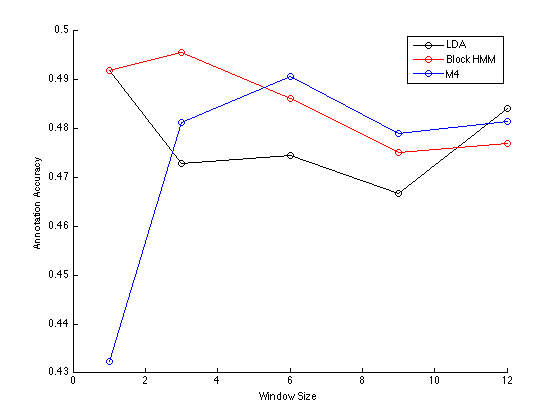
\includegraphics[width=0.7\textwidth]{experiment1_1.png}
    \caption{Experiment 1 (Negotiation framework). The Y-axis denotes the annotation accuracy (F1 score), whereas the X-axis denotes the window size ($k$) of the turns that we consider.}
  \label{fig:experiment1_1}
\end{figure}

As seen in Figure \ref{fig:experiment1_1}, there does not seem to be a significant performance difference between the three models on the annotation task in the negotiation framework. While the M4 model performs significantly worse than other models when $k = 1$, the performance of the M4 model improves when I increase the window size. This indicates that the information from the preceeding and the following turns do help the M4 model with the prediction. Note that all of the models significantly outperform the chance ($=20 \%)$. I conclude that while the topic distributions of each turn can be a good feature to predict the label in the negotiation framework, it is hard to evaluate which model worked better in relative to other models based on the negotiation prediction accuracy.


\subsection{Annotation Prediction Using the Topic Distributions: Heteroglossia Framework}

Again, I assume that a good topic model will be able to predict the annotations from the Heteroglossia Framework. Using the similar approach as above, I obtain the following results.

\begin{figure}[h!]
  \centering
    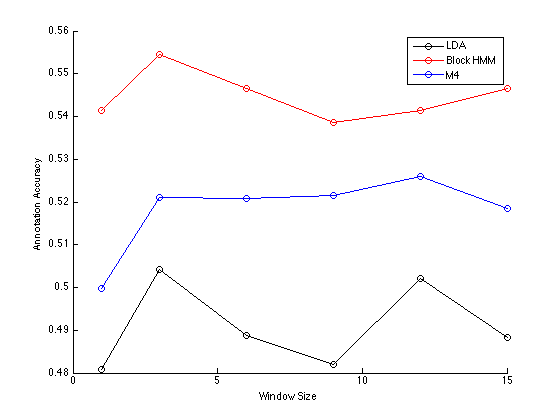
\includegraphics[width=0.7\textwidth]{experiment1_2.png}
    \caption{Experiment 2 (Heteroglossia framework). The Y-axis denotes the annotation accuracy (F1 score), whereas the X-axis denotes the window size ($k$) of the turns that we consider.}
  \label{fig:experiment1_2}
\end{figure}

In Figure \ref{fig:experiment1_2}, the Block HMM model outperforms the other two models for every window size that we have tried. All of the models peak at $k=3$, which looks at the immediately preceeding turn and the following turn to predict the label for the current turn. Note that all of the models significantly outperform the chance ($=25 \%$). I conclude that while the topic distributions of each turn can be a good feature to predict the label in the Heteroglossia framework, the Block HMM model performs significantly better than the other two models.

\pagebreak

\subsection{Topic Coherence}

In this experiment, I evaluate each topic model by evaluating the coherence of the representative (top-ranked) words from each model. I assume that the top-ranked words from different topic clusters should be distinctly coherent. While it would be also interesting to sub-categorize the words by their speakers or sessions, I only consider the plain output from each of the model. Tables \ref{tab:block} and \ref{tab:m4} show the results.

Each column of the table represents the top 10 words from each topic cluster. However, it is not clear whether the topics are distinctly categorized and whether the words in the same cluster are coherent for any of the two models that I compared (Block HMM and M4). 

\begin{table*}
    \begin{center}
    \caption{Top 15 words for each topic from the Block HMM model}
    \begin{tabular}{ccccc}
        \hline
        1 & 2 & 3 & 4 & 5 \\
        \hline
        are & happen & a & write & solution  \\
        video & glucose & for & now & video  \\
        do & that & when & watch & water  \\
        who & what & mates & condition & desktop  \\
        so & think & one & observed & watch  \\
        for & each & team & conditions & folder  \\
        should & was & so & are & videos  \\
        a & a & example & video & and  \\
        and & and & encourage & b & glucose  \\
        condition & it & your & what & starch  \\
        this & water & would & the & replace  \\
        your & you & do & and & with  \\
        what & for & what & your & a  \\
        \hline
    \end{tabular}
    \end{center}
    \label{tab:block}
\end{table*}

\begin{table*}
    \begin{center}
    \caption{Top 15 words for each topic from the M4 model}
    \begin{tabular}{ccccc}
        \hline
        1 & 2 & 3 & 4 & 5 \\
        \hline
        think & write & how & benefit & specific  \\
        was & solution & discuss & asking & looking  \\
        so & starch & from & was & make  \\
        water & happen & back & whether & it  \\
        do & you & different & being & both  \\
        are & now & move & please & talking  \\
        video & with & predictions. & them & sure  \\
        it & will & compare & get & water  \\
        a & cell & now & when & responsible  \\
        for & and & you & mates & nice  \\
        your & c & a & team & all.  \\
        and & b & about & encourage & you  \\
        what & glucose & condition & example & each  \\
        you & condition & observed & one & for  \\
        \hline
    \end{tabular}
    \end{center}
    \label{tab:m4}
\end{table*}
\end{document}
